% ACHTUNG: Für das Erstellen des Literaturverzeichnisses wird das modernere Paket biblatex
%			 in Kombination mit biber verwendet -- nicht mehr das ältere BibTex!
% 			 Bitte stellen Sie ggf. Ihre TeX-Umgebung
% 			 entsprechend ein (z.B. TeXStudio: Einstellungen --> Erzeugen --> Standard Bibliographieprogramm: biber)
%

\documentclass[
	12pt,
	BCOR=5mm,
	DIV=12,
	headinclude=on,
	footinclude=off,
	parskip=half,
	bibliography=totoc,
	listof=entryprefix,
	toc=listof,
	pointlessnumbers,
	plainfootsepline]{scrreprt}

%	Konfigurationsdatei einziehen
\input{config}
\usepackage{pdfpages}

\begin{document}

%% BITTE GEBEN SIE HIER DEN TITEL UND DIE AUTORIN / DEN AUTOR DER ARBEIT AN!
%% DIESE INFORMATIONEN _MÜSSEN_ GESETZT SEIN, UM TITELBLATT, ABSTRACT UND
%% EIGENSTÄNDIGKEITSERKLÄRUNG AUTOMATISCH ANZUPASSEN!
\TitelDerArbeit{Möglichkeiten zum personalisierten Lernen im Studium}
\AutorDerArbeit{Andrea Engel}
\Firma{SAP SE}
\Kurs{WWI 17 SEB}

\begin{titlepage}
\begin{minipage}{\textwidth}
		\vspace{-2cm}
		\noindent \includegraphics[scale=0.14]{img/sap.png} \hfill   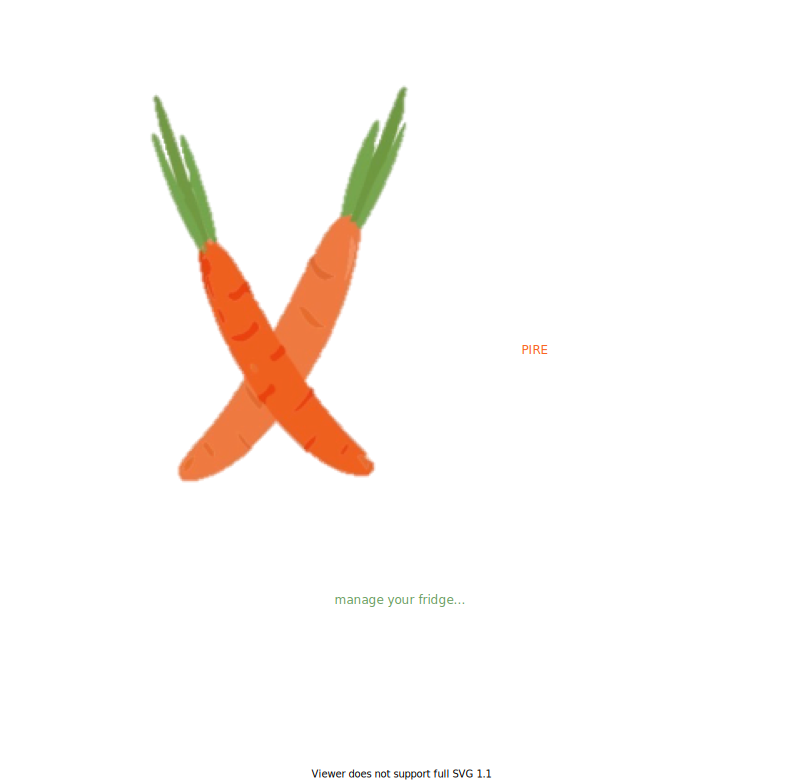
\includegraphics{img/logo.jpg}
\end{minipage}
\vspace{1em}
\sffamily
\begin{center}
	\textsf{\large{}Duale Hochschule Baden-W\"urttemberg\\[1.5mm] Mannheim}\\[2em]
	\textsf{\textbf{Seminararbeit}}\\[8mm]
	\textsf{\textbf{\Large{}Xpire - Dokumentation zum Projekthergang}} \\[1.5cm]
	\textsf{\textbf{\Large{}Studiengang Wirtschaftsinformatik}\\[3mm] \textsf{Studienrichtung Software Engineering}}
	
	\vspace{3em}
%	\textsf{\Large{Sperrvermerk}}
\vfill

\begin{minipage}{\textwidth}

\begin{tabbing}
	Wissenschaftlicher Betreuer: \hspace{0.85cm}\=\kill
	Verfasser: 
		\> Engel, Andrea: xyz \\
		\> Dutzi, Jonas: 6681598 \\
		\> Richarz, Verena: xyz \\
		\> Waage, Felix: 3459154 \\
		\> Werner, Yvonne: 8519757 \\
		\> Westphal, Fabio: 6198411 \\
		\> Zahn, Milena: 7488221 \\\\
	Firma: \> SAP SE \\[1.5mm]
	Kurs: \> WWI 17 SEB\\[1.5mm]
	Studiengangsleiter: \> Prof. Dr. Sebastian Ritterbusch  \\[1.5mm]
	Modul: \> Entwicklung mobiler Applikationen \\[1.5mm]
	Dozent/-in: \> Michael Spengler \\[1.5mm]
	Bearbeitungszeitraum: \> 11.05.2020 - 31.07.2020
	
\end{tabbing}
\end{minipage}

\end{center}

\end{titlepage}

\pagenumbering{roman} % Römische Seitennummerierung
\normalfont

%--------------------------------
% Verzeichnisse - nicht benötige Verzeichnisse bitte auskommentieren / löschen.
%--------------------------------

%   Sperrvermerk
%\chapter*{}
Die nachfolgende Arbeit enthält vertrauliche Daten der:

\vspace{0.5cm}

	SAP SE
	
	Dietmar-Hopp-Allee 16
	
	69190 Walldorf
	
\vspace{0.5cm}
Der Inhalt dieser Arbeit darf weder als Ganzes noch in Auszügen Personen außerhalb des Prüfungsprozesses und des Evaluationsverfahrens zugänglich gemacht werden, sofern keine anders lautende Genehmigung der Ausbildungsstätte vorliegt. 
\cleardoublepage


% Ehrenwörtliche Erklärung ewerkl.tex einziehen
% \input{ewerkl.tex}

%	Kurzfassung
% \input{abstract}

%	Inhaltsverzeichnis
\tableofcontents

%	Abbildungsverzeichnis
%\listoffigures

%	Tabellenverzeichnis
% \listoftables

%	Listingsverzeichnis
% \lstlistoflistings

% 	Algorithmenverzeichnis
%\listofalgorithms

% 	Abkürzungsverzeichnis (siehe Datei acronyms.tex!)
% !TEX root =  master.tex

\clearpage
\chapter*{Abkürzungsverzeichnis}	
\addcontentsline{toc}{chapter}{Abkürzungsverzeichnis}


\begin{acronym}
	\acro{DHBW}{Duale Hochschule Baden-Württemberg}
	\acro{PWA}{Progressive Web App}
	\acro{VPC}{Values Proposition Canvas}
	\acro{MVP}{Minimal Viable Product}

\end{acronym}


%--------------------------------
% Start des Textteils der Arbeit
%--------------------------------
\clearpage
\ihead{\chaptername~\thechapter} % Neue Header-Definition
\pagenumbering{arabic}  % Arabische Seitenzahlen

%	Anleitungs-Datei anleitung.tex einziehen. Auf diese Weise sollten Sie versuchen, für jedes einzelne
% Kapitel eine eigene Datei anzulegen und mittels input-Kommando einzuziehen.

% !TEX root =  master.tex
\chapter{Einleitung}
% Random commentar
\input{tex/chapter01/1.1.grundidee}
% !TEX root =  master.tex
\section{Was ist eine PWA?}
% !TEX root =  master.tex
\section{Vorgehensweise}
Um so effektiv wie möglich zusammen zuarbeiten, haben wir uns eine flexible Art der Aufgabenaufteilung überlegt. Dabei sind wir wie folgt vorgegangen: Zunächst haben wir gemeinsam in einer Brainstorming-Session überlegt, welche Funktionalitäten die Xpire-App beinhalten soll, wie sie aussehen soll und welche Technologien wir für die Umsetzung verwenden möchten. Anschließend hat sich jedes Gruppenmitglied selbstständig mit den Grundlagen einer PWA als auch mit der Softwarebibliothek React vertraut gemacht. In einer zweiten Session haben wir gemeinsam die Code-Basis für das Projekt aufgesetzt und jeder Person je nach individuellen Stärken und Interessen eine spezifische Verantwortlichkeit im Projekt zugeteilt. Dabei sei gesagt, dass eine Person nicht zwangsläufig nur im eigenen Verantwortungsbereich agieren muss. Jeder darf entsprechend seiner Stärken den Fokus setzen und darüber hinaus weiteren Aufgaben außerhalb seines Schwerpunktes nachgehen und die anderen Team-Mitglieder bei ihren Aufgaben unterstützen. Wichtig ist uns, dass sich jeder im Team wohl fühlt, dem nachgehen kann, worauf er Lust hat und, ganz wichtig, durch Learning-by-Doing ganz viel Neues erlernen kann.\\
Die Schwerpunkte pro Teammitglied wurden wie folgt verteilt:
\begin{itemize}[noitemsep]
	\item \textbf{Felix:} Projektleitung, PWA, ...
	\item \textbf{Fabio:} Datenbank,...
	\item \textbf{Jonas:} React, 
	\item \textbf{Verena:} Mockups, React, ...
	\item \textbf{Milena:} 
	\item \textbf{Yvonne:}
	\item \textbf{Andrea:} Logo-Design, Mockups, Dokumentation
\end{itemize}
Freitags, an unseren offiziellen Meeting-Terminen, stellen wir einander vor, welche Aufgaben in der Zwischenzeit umgesetzt wurden, definieren neue Aufgaben und reflektieren die bisherige Vorgehensweise. Unter der Woche vereinbaren wir je nach Bedarf individuell Termine mit dem gesamten Team oder treffen uns in Teilgruppen, um bestimmte Aufgaben umzusetzen.\\
Das gesamte Projekt kennzeichnet sich daher durch eine iterativen Arbeitsweise, sodass genug Platz für neue Ideen und Erweiterungen bleibt. Ziel ist es, zunächst ein Minimal-Viable-Product (MVP) zu entwickeln, um ein funktionierendes Produkt liefern zu können, welche sich in zukünftigen Schritten einfach erweitern lässt.



% !TEX root =  master.tex
\chapter{Analyse}

% !TEX root =  master.tex
\section{Value Proposition Canvas}
Ein Value Proposition Canvas (VPC) stellt eine Ergänzung zum Business Model dar und ist ein Werkzeug, welches das Designen, Testen, Verwalten und Erstellen von Kundenwertversprechen unterstützt. \enquote{Think of the Value Proposition as a contract between the customer and your company where the customer “hires” your company to solve a problem.} (Clayton Christensen) Mit dieser Formulierung bringt Christensen ziemlich genau auf den Punkt, was man unter einem VPC versteht. Es bildet gewissermaßen einen Vertrag zwischen Kunde und Unternehmen, indem es darum geht, ein Problem des Kunden zu lösen. Das VPC hilft nicht nur systematisch das Wertversprechen des Unternehmens herauszuarbeiten, es ist auch Basis für Marketing, Pricing und den späteren Erfolg am Markt. Aus einer Umfrage von Simon \& Kucher aus dem Jahr 2014 geht hervor, dass 72\% aller Produktinnovationen scheitern. Hauptgrund dafür ist die fehlende Wahrnehmung beim Kunden.\autocite[vgl.][]{Simon&Kucher.2014}\\
\begin{figure}[htbp] 
	\centering
	\includegraphics[width=0.8\textwidth]{img/VPC.pdf}
	\caption{Value Proposition Canvas}
	\label{fig:vpc}
\end{figure}

Die Abbildung \ref{fig:vpc} zeigt den Value Proposition Canvas für die Xpire-App. Dabei stehen sich Wertversprechen der App und die das Kundenprofil gegenüber. Die Kundenseite gliedert sich in \enquote{Customer Jobs}, \enquote{Gains} und \enquote{Pains}. Dadurch wird aufgezeigt, welche Aufgaben der Kunde erledigen möchte, warum er diese erledigen möchte und mit welchen Herausforderungen und Schwierigkeiten er dabei konfrontiert wird. Auf der linken Seite des VPC sind die Wertversprechen des Unternehmens zu sehen, unterteilt in \enquote{Gain Creator}, \enquote{Pain Relievers} und \enquote{Products \& Services}.\\
Im gewählten Beispiel ist der Kunde ein Student namens Karl, der in einer Wohngemeinschaft wohnt und daher einen Kühlschrank mit seinen Mitbewohnern teilt. Er geht häufig einkaufen, hat meistens Geldprobleme und einen schlechten Überblick über seine Lebensmittel, da er oft gestresst oder unterwegs ist. Zu seinen Jobs (im Haushalt) gehört das regelmäßige Überprüfen des Kühlschranks und das Verwerten der Lebensmittel, bevor sie abgelaufen sind. Leider gelingt ihm das meistens nicht, weshalb er regelmäßig verdorbene Lebensmittel wegwerfen muss. Dies ist nicht nur eine Form der Lebensmittel- sondern auch der Geldverschwendung und führt bei Karl regelmäßig zu Frust und einem schlechten Gewissen. Zusätzlich ärgern sich seine Mitbewohner über den Gestank im Kühlschrank, wenn mal wieder ein Produkt verschimmelt ist und Karl muss öfter als ihm lieb ist den Kühlschrank putzen. Er wünscht sich, weniger verschwenderisch zu leben mehr Kontrolle über den Stand seiner Lebensmittel zu haben. Er möchte ein gutes Gewissen haben, wenn es um seine Finanzen geht und verantwortungsvoll im Umgang mit Nahrungsmitteln sein.\\
Die mobile Applikation \enquote{Xpire} hilft Karl seine Ziele zu erreichen und sein Verhalten bezüglich der Lebensmittel- und Geldverschwendung zu verbessern. Xpire ermöglicht ihm eine schnelle und einfache Übersicht über den Stand aller seiner Lebensmittel. Zusätzlich erhält er rechtzeitig Hinweise, wenn eines seiner Lebensmittel kurz vor dem Ablauf der Haltbarkeit steht. Karl hat somit die volle Kontrolle über all seine Lebensmittel und kann nun weniger verschwenderisch leben. Das schont nicht nur seinen Geldbeutel, auch sein Gewissen und seine Mitbewohner freuen sich. Gestank und verschimmeltes Essen im Kühlschrank gehören nun der Vergangenheit an.\\
Mit Xpire können alle gekauften Produkte in der App eingescannt oder manuell hinterlegt werden. Die Produktdaten werden anschließend in einer Datenbank gespeichert. Zu jedem Produkt können zusätzliche Informationen wie Menge, Einkaufsdatum und Verfallsdatum hinterlegt werden. Die Hauptfunktionalität von Xpire besteht darin, dem Benutzer auf übersichtliche Art und Weise all seine hinterlegten Produkte anzuzeigen und ihn per Push-Notifications eine Erinnerung zu schicken, wenn eines seiner Produkte kurz vor dem Ablauf des Haltbarkeitsdatums steht. Zukünftige Features sollen Rezeptvorschläge und Hinweise zu Nährwerten enthalten. 

% Monetarisierungsoption? Über Werbung? Premium Account?

% !TEX root =  master.tex
\section{Benutzerprofilanalyse}
Im Rahmen der Benutzerprofilanalyse werden die Eigenschaften der Endanwender untersucht, um die Gebrauchstauglichkeit der Anwendung sicherzustellen. Eine wesentliche
Rolle spielen dabei die persönlichen Merkmale, Fähigkeiten und Kenntnisse der Benutzer
sowie deren Einordnung in ein bestimmtes Nutzungsverhalten.\\
Da die progressive Web App von möglichst vielen Nutzern verwendet werden soll, gibt es kaum Einschränkungen, was die Zielgruppe betrifft. Die Gemeinsamkeit der Nutzer liegt im Besitz eines Kühlschrankes, dem selbstständigem Tätigen von Lebensmittel-Einkäufen sowie im Besitz eines Smartphones oder eines Computers. Daraus lässt sich ableiten, dass die Zielgruppe überwiegend volljährig ist und ein Smartphone oder einen Computer besitzt. Laut Statista besitzen aktuell 66,5 Mio Menschen in Deutschland ein Smartphone.\footnote{\url{https://de.statista.com/statistik/daten/studie/500579/umfrage/prognose-zur-anzahl-der-smartphonenutzer-in-deutschland/}} Ca. 13 Mio Menschen in Deutschland sind Minderjährig, wobei nicht alle Minderjährigen ein Smartphone besitzen. Zieht man trotzdem die Anzahl aller Minderjährigen von der Anzahl der Menschen, die in Deutschland ein Smartphone besitzen, ab, kommt man immer noch auf eine Anzahl von mindestens 49 Mio potentiellen Nutzer. Das sind  mehr als 50\% aller deutschen Staatsbürger.\\
All diese Nutzer können einen völlig unterschiedlichen Erfahrungsschatz bezüglich der Nutzung von neuen Technologien aufweisen. Von der Rentnerin, die nur selten einen Computer verwendet bis hin zum zwanzigjährigen Studierenden, der selbstständig Web Apps programmiert, können die unterschiedlichsten Ausgangsvoraussetzungen gegeben sein. Es is davon auszugehen, dass ein Großteil der Anwendet eine durchschnittliche Technikaffinität aufweist, es aber auch Anwender gibt, die keinerlei oder kaum Erfahrungen im Umgang mit Web Apps aufweisen. Demzufolge sollte die Oberfläche gleichzeitig so konzipiert sein, dass sie auch für Laien intuitiv und verständlich ist. Ein strukturierter und klarer Aufbau könnten diesem Aspekt Rechnung tragen. Schließlich sei noch zu erwähnen, dass die Web App vorerst nur für Deutschland entwickelt wird. Zu einem späteren Zeitpunkt ist die Internationalisierung der Applikation durchaus denkbar, dafür bedarf es dann einer Möglichkeit zur Auswahl unterschiedlicher Sprachen.




% !TEX root =  master.tex
\section{Anforderungsanalyse}
% !TEX root =  master.tex
\section{Monetarisierungsstrategie}
% kostenlos -> viele sollen die App nutzen
% Zusatz: 
%	- Angebote von Supermärkten
%	- Rezeptvorschläge für die Produkte die ablaufen
% Monetarisierung: freiwillige Spenden, Kooperation mit Chefkoch, Supermärkten, restegourmet etc.
% Schalten von werung: darf aber nicht unseriös, aufdringlich oder nervig wirken -> Webrung muss gegen Bezahlung deaktiviert werden können
% nicht alle Möglichkeiten können gleichzeitig umgesetzt werden

% am Ende: keine Werbung -> Finanzierung durch Spenden
% gemeinnütziges Projekt -> Kostenlose Infrastruktur zB bei Strato

% !TEX root =  master.tex
\chapter{Konzeption und Entwurf}

\section{Eingesetzte Technologien}

\section{Konzeptuelles Modell}

\section{Entwicklung von Prototypen}

% !TEX root =  master.tex
\section{Eingesetzte Technologien}


% !TEX root =  master.tex
\section{Konzeptuelles Modell}
% Welche Architektur und Warum?
% User-Authentifizierung?
% Welche Persistierung?
% Welche Tests und warum?

In den vorherigen Abschnitten wurden bereits einige Merkmale der Xpire-App beschrieben, allerdings wurden die Zusammenhänger der verschiedenen Bestandteile nicht näher erläutert, weshalb in diesem Abschnitt das konzeptionelle Modell näher erklärt wird. 

Kern der Xpire-App ist das Frontend, welches mit Hilfe von React als PWA konzipiert ist. Wie den Abbildungen \ref{fig:prot1} und \ref{fig:prot2} entnommen werden kann, besteht die Xpire-App aus 3 Ansichten: \textit{Home-Screen}, \textit{Product-Screen} und dem \textit{Create-Screen}. Diese Ansichten werden in React durch Komponenten realisiert, welche in unterschiedlichen Kontexten wiederverwendet werden können. Der Home-Screen besitzt so die AppBar und eine Komponente zur Listendarstellung der Produkte. Die Ansichten \textit{Product-Screen} und \textit{Create-Screen} werden durch die selbe Komponente realisiert, da zum Erstellen und Anzeigen der Produktinformation ähnliche UI-Bestandteile benötigt werden. Die Darstellung passt sich hierbei automatisch anhand der Übergebenen Parameter an. Hierdurch können Code-Duplikate vermieden werden und auch der Raum für Fehler wird reduziert. 

Ein Weiterer wichtiger Bestandteil der Anwendung ist die IndexedDB, welche zur dauerhaften Persistierung der Daten verwendet wird. Wie bereits in Abschnitt \ref{chapter:datenbank} erwähnt wird hierfür das Modul \textit{Dexie} verwendet. Neben der Datenhaltung in der lokalen Datenbank wird eine aktuelle Kopie der gesamten Datenbank in einem Array im \textit{State} der App-Komponente synchron gehalten, wodurch sowohl die Listen-Komponente als auch die Product-Screen-Komponente darauf zugreifen können.

Der Nutzer soll später seine Produkte mit Hilfe des einheitlichen Barcodes hinzufügen können. Dies soll die Verwendung deutlich beschleunigen und vereinfachen, da so Informationen wie Titel, Gewicht, usw. nicht manuell eingetragen werden müssen. Um die dazu benötigten Informationen zu erhalten wird die OpenFoodFacts-Api verwendet. Diese führt eine Datenbank mit umfassenden Produktinformationen und kann Anfragen über den Barcode entgegennehmen. Des Weiteren wird diese Api verwendet um Abbildungen der einzelnen Produkte zu erhalten, wodurch dem Nutzer die Verwendung der Anwendung weiter vereinfacht werden soll. In einer späteren Version ist es darüber hinaus angedacht die Porduktbilder lokal in der Datenbank zu speichern, um auch bei Offlinebetrieb Bilder anzeigen zu können.
% !TEX root =  master.tex
\section{Entwicklung von Prototypen}
\subsection{Figma}
Zur Erstellung der Prototypen haben wir das Design-Tool \enquote{Figma} verwendet. Dies ist ein Kollaborations-Tool für Designer und funktioniert ähnlich wie Sketch oder Adobe XD, zeichnet sich aber durch zwei signifikante Unterschiede aus\autocite[vgl.][]{?}:
\begin{itemize}[noitemsep]
	\item Es läuft zu 100 \% in Ihrem Browser (keine Installation nötig)
	\item Möglichkeit der Kollaboration mit anderen Personen in Echtzeit
\end{itemize}
Dadurch liefert Figma viele Vorteile, die das gemeinsame Erstellen von Prototypen stark verbessern. Das Tool ist von Designern für Designer entwickelt wurden und einfach im handling. Benutzeroberflächen lassen sich schnell und effektiv designen, ohne viel Zeit in die Einarbeitung des Tools investieren zu müssen. Das kollaboratives Arbeiten in Echtzeit ermöglicht die unkomplizierte Zusammenarbeit am selben Entwurf, ohne extra ein Tool zu installieren oder sich physisch treffen zu müssen. Des weiteren bietet Figma die Möglichkeit, erstellte Screens in vier verschiedenen Formaten zu exportieren als auch Interaktionen hinzuzufügen, um das Projekt im Live-Preview betrachten zu können. Im Live-Preview lassen sich alle zuvor definierten Interaktionen, wie beispielsweise das Navigieren auf einen anderen Screen, ausprobieren und imitieren das Feeling einer echten Anwendung.

\subsection{Mobile First}
Da unsere Zielgruppe eine breite Masse an Menschen beinhaltet, haben wir wert darauf gelegt, dass Xpire möglichst einfach und unkompliziert verwendet werden kann. Einem ansprechenden User Interface sowie einer intuitive User Experience werden daher besondere Bedeutung zugeschrieben.\\
Im Jahr 2015 meldete Google erstmals, dass mehr Suchanfragen über mobile Endgeräte als über Desktop-Geräte erfolgten. Seitdem steigt die der Anteil der Internetnutzer, die auch mit dem Smartphone online gehen, rapide. \footnote{\url{https://de.statista.com/statistik/daten/studie/633698/umfrage/anteil-der-mobilen-internetnutzer-in-deutschland/}} Resultierende aus dieser Entwicklung ist die Wahl des Mobile-First-Ansatzes selbsterklärend. Inzwischen ist nicht mobil-optimierter (responsive) Content ist kaum noch vorstellbar. Mobile Frist lässt sich als neuer Denkansatz im Webdesign definieren. Das Design einer Website wird dabei erstmal in der mobilen Version optimiert, bevor es für größere Bildschirme entwickelt wird. Man arbeitet also von der kleinsten Layout-Version hin zur größten.\autocite[vgl.][]{?}

% Schrittfolge der Screens erklären
\begin{figure}[hbt!]
	\centering
	\includegraphics[width=1.0\textwidth]{img/Prototype_01.pdf}
	\caption{Xpire Welcome-Screen und Home-Screen}
	\label{fig:prot1}
\end{figure}
Die Abbildung \ref{fig:prot1} zeigt den Welcome-Screen und den Home-Screen der Xpire-App.


\begin{figure} 
	\centering
	\includegraphics[width=1.0\textwidth]{img/Prototpye_02.pdf}
	\caption{Xpire Delete-Screen und Product-Screen}
	\label{fig:prot2}
\end{figure}

% !TEX root =  master.tex
\chapter{Präsentation der PWA}
In diesem Kapitel wird die umgesetzte PWA, die zuvor durch Mockups dargestellt wurde, vorgestellt. Da die Grundlagen zur Technologie bereits im Kapitel 3 ausführlich erläutert worden sind, wird hier nicht mehr näher auf die Implementierungsdetails eingegangen,
sondern lediglich das Resultat anhand von Screenshots vorgestellt. Abschließend findet noch ein Abgleich mit den zuvor definierten Anforderungen statt.

Die Umsetzung der PWA erfolgte mithilfe der JavaScript-
Bibliothek React auf Basis des entwickelten Prototypen. Im Folgenden wird der aktuelle Entwicklungsstand
der App näher vorgestellt. Dabei wird auf die Gestaltung
und die Navigation als auch auf die Funktionalität der PWA eingegangen.

\begin{figure}[h!]
	\centering
	\includegraphics[width=1.0\textwidth]{img/app.pdf}
	\caption{Xpire auf Laptop vs. Smartphone}
	\label{fig:app}
\end{figure}

%\begin{wrapfigure}{r}{0.5\textwidth}
%	\vspace{-1.5\baselineskip}
%	\begin{center}
%		\includegraphics[width=0.50\textwidth]{img/plus.jpg}
%	\end{center}
%	\setcapindent{0cm}
%	\caption{Ausschnitt des ungerichteten Graphen zum %Einkauf-Problem}
%	\label{fig:graph_edeka}
%\end{wrapfigure}

Die Abbildung \ref{fig:app} zeigt, wie sich die Xpire-App verschiedenen Bildschirmgrößen problemlos anpasst. Zu sehen ist der \textit{Home-Screen} mit einer Auswahl an Beispiel-Produkten sowohl auf dem Laptop als auch auf dem Smartphone.\\
Um Xpire auf dem Laptop zu installieren, muss man folgenden Link in die Adresszeile seines Browsers eingeben: https://felixwaage.github.io/Xpire/. Es erscheint die App,  wie zu sehen in Abbildung \ref{fig:install} im Browser und lässt sich über ein "+" ganz rechts in der Adresszeile als App dem Desktop hinzufügen. Nach einem Klick auf den Plus-Button öffnet sich ein Pop-Up, welches es dem Nutzer ermöglicht, die Installation durchzuführen. Klick man den Installations-Button, wird im dritten Schritt die Xpire-App auf dem Desktop hinterlegt, siehe \ref{fig:install}.

\begin{figure}[h!]
	\centering
	\includegraphics[width=1.1\textwidth]{img/install.pdf}
	\caption{Xpire-Installationsprozess am Laptop}
	\label{fig:install}
\end{figure}

Die Installation auf dem Smartphone erfolgt äquivalent zu der auf dem Desktop. Nach dem Öffnen des Links wid über ein Pop-Up die Möglichkeit zur Installation bereit gestellt. Xpire wird dann auf dem Smartphone angezeigt wie eine native mobile App und weist auch nach dem Öffnen keine Unterschiede zu einer nativen App auf. Dennoch läuft die App als PWA komplett im Browser. 

Damit die User Experience der PWA-Applikation auf dem Smartphone ähnlich zu einer nativen Applikation ist, wird ein sogenannter Splash Screen implementiert. Dieser erscheint nachdem der Benutzer die auf dem Smartphone gespeicherte Xprie-PWA öffnet. In Abbildung \vref{fig:splashScreen} werden die Splash Screens abgebildet, wobei dieser bei einem iOS-Betriebssysteme in weiß und für Android-Geräte in grün erscheint.  

Der Splash Screen sowie weitere Funktionalität der Xpire-Applikation sind in einer Bildschirmaufnahme mit dem Betriebssystem iOS zu sehen, welche unter folgendem Link verfügbar ist:\\
\url{https://github.com/felixwaage/Xpire/blob/master/iOS-Bildschirmaufnahme.mov} 

\begin{figure}[H]
	\centering
	\subfigure[iOS]{\includegraphics[width=0.30\textwidth]{img/splashScreenIos.png}} 
	\subfigure[Android]{\includegraphics[width=0.30\textwidth]{img/splashScreenAndroid.jpg}} 
	\caption{Splash Screen für iOS und Android}
	\label{fig:splashScreen}
\end{figure}

% was ist unterschiedlich im Vergleich zu den Mockups?
Die Gestaltung als auch der User-Flow der entwickelten PWA entsprechen fast eins zu eins dem der Mockups. Geringe Unterschiede lassen sich an folgenden Punkten feststellen:
 \begin{itemize}[noitemsep]
 	\item \textbf{AppBar:} Das Logo in der entwickelten PWA hat einen weißen Kreis als Hintergrund. Das Icon oben recht ist nicht wie im Mockup ein Zahnrad, sondern ein weißes Mülleimer-Icon.
 	\item \textbf{Produkt löschen:} Die Produkte lassen sich einzeln nicht direkt im \textit{Home-Screen} per Wischen nach links, wie designed im Mockup, löschen, sondern lediglich im \textit{Produkt-Screen} über ein Mülleimer-Icon. Wird jedoch das Mülleimer-Icon oben rechts in der AppBar des \textit{Home-Screen} dar, erhält der Nutzer die Möglichkeit, alle hinterlegten Produkte auf einmal zu löschen.
 	\item \textbf{Produkte verwalten:} Der \textit{Produkt-Screen} wurde implementiert, so wie er im Mockup designed wurde. Das hinterlegte Bild wird angezeigt und Name, Anzahl, Einkaufsdatum und Ablaufdatum lassen sich durch das Anklicken des jeweiligen Textfeldes ändern. Lediglich die Terminologie des Buttons hat wurde von \enquote{Speichern} zu \enquote{Ändern} verändert.
 \end{itemize}

%neuer Screen: Produkt hinzufügen 
Neben der Umsetzung des erstellten Mockups, wurde zusätzlich eine Ansicht zum Hinzufügen eines neuen Produktes entwickelt, zu sehen in Abbildung \ref{fig:add}. Der Nutzer hat die Möglichkeit einen Barcode zu scannen oder ihn manuell im Barcode-Textfeld einzugeben. Über die OpenFood-API wird automatisch das jeweilige Produktbild angezeigt und der Titel im dazugehörigen Feld angezeigt.

\begin{figure}[h!]
	\centering
	\includegraphics[width=0.6\textwidth]{img/add.pdf}
	\caption{Produkt hinzufügen}
	\label{fig:add}
\end{figure}

Die Standard-Anzahl der Produkte beträgt 1, lässt sich aber über ein Dropdown einfach erhöhen. In dem Eingabefeld für das Einkaufsdatum ist automatisch das aktuelle Datum vorausgewählt, was sich jedoch ändern lässt, sobald man in das Textfeld reinklickt. Es öffnet sich ein Date-Picker, genau wie bei der Eingabe des Gültigkeitsdatums. Nach dem Speichern wird das Produkt automatisch dem \textit{Home-Screen} hinzugefügt.


% Tests --> feingarnulare Unit Tests, acceptance tests?


% !TEX root =  master.tex
\section{Präsentation der entwickelten PWA}
Die Umsetzung der PWA erfolgte mithilfe der JavaScript-
Bibliothek React auf Basis des entwickelten Prototypen. Anhand von Screenshots soll im Folgenden der aktuelle Entwicklungsstand
der App näher vorgestellt werden. Dabei wird auf die Gestaltung
und die Navigation als auch auf die Funktionalität der PWA eingegangen.

\begin{figure}[h!]
	\centering
	\includegraphics[width=1.0\textwidth]{img/app.pdf}
	\caption{Xpire auf Laptop vs. Smartphone}
	\label{fig:app}
\end{figure}

Die Abbildung \ref{fig:app} zeigt, wie sich die Xpire-App verschiedenen Bildschirmgrößen problemlos anpasst. Zu sehen ist der \textit{Home-Screen} mit eine Auswahl an Beispiel-Produkten.\\



% allgemeine Vorstellung -> Respnsiveness

% Installation

% Tests --> feingarnulare Unit Tests, acceptance tests?

% Deployment
% !TEX root =  master.tex
\section{Anforderungsabgleich}

% Welche Tests und warum?
% Welche Persistierung

% !TEX root =  master.tex
\chapter{Zusammenfassung und Ausblick}

% Was könnten nächste Schritte sein? Wie könnte die App erweitert werden?

% Was passiert, wenn man ein Produkt löscht? Ist es dann in der Datenbank geschlöscht oder wird nur ein Attribut gesetzt? Welche Auswirkungen hätten diese Möglichkeiten?

% Was waren unsere Learnings?


%	Literaturverzeichnis
\ihead{} % Neue Header-Definition
\printbibliography
\cleardoublepage

% Der Anhang beginnt hier - jedes Kapitel wird alphabetisch aufgezählt. (Anhang A, B usw.)
\appendix
\ihead{\appendixname~\thechapter} % Neue Header-Definition

% appendix.tex einziehen
\input{appendix}


\end{document}
